\documentclass[]{article}
\usepackage{polski}
\usepackage[utf8]{inputenc}
\usepackage{mathtools}
\usepackage{pgfplots}
\usepackage{listings}
\usepackage{enumitem}
\usepackage{mathtools}
\usepackage{amsmath}
\usepackage{amssymb}
\usepackage{pgf,tikz}
\usepackage{mathrsfs}
\usetikzlibrary{arrows}
%opening
\let\normalint\int % PS
\def\int{\displaystyle\normalint} %PS
\title{\textbf{ Metody Numeryczne 2\\Laboratorium 4\\}
Aproksymacja średniokwadratowa ciągła w przestrzeni $L_p^2(-1,1) dla p(x)=1/(sqrt(1-x^2))$ w bazie wielomianow Czebyszewa. }
\author{Szymon Adach}

\begin{document}

\maketitle


\section{Treść zadania}
 \textbf{Zadanie 11:} Obliczanie całek ${\displaystyle \iint\limits_D f(x,y) \,dx\,dy}$ gdzie $D=\{(x,y) : \varphi(x,y) \leqslant 0\}$
\section{Opis metody}
Metoda polega na losowaniu wartości $(x, y, z) \in [a, b] \times [c, d] \times [0, M] \\(0 \leq f(x,y) \leq M)$ oraz inkrementowaniu wskaźników: 
\begin{itemize}
	\item \textbf{ll} - liczba wszystkich losowań oraz 
	\item \textbf{ls} - liczba losowań takich, że $(x,y) \in D \land z \leq f(x,y)$.
\end{itemize}
Wówczas obliczana metodą Monte-Carlo wartość całki wynosi:
\begin{center}
	$S(f) = \frac{ls}{ll}\cdot(b-a)\cdot(d-c)\cdot M$
\end{center}
Pętla główna programu ma postać:
\begin{lstlisting}[mathescape, language=Matlab]
for k = 1:max_iter
	ll = ll + 1;
	x = a + rand(1) * (b - a);
	y = c + rand(1) * (d - c);
	z = rand(1) * M;
	
	if(area(x, y) <= 0 &&  z < func(x,y))
		ls = ls + 1;
	end
	
	if(mod(k, interval) == 0)
		val = ls / ll * (b - a)*(d - c) * M;
		fprintf('Wartosc po %d iteracjach: %f\n', k, val);
	end;
end
\end{lstlisting}
\section{Działanie programu}

Program jest uruchamiany poleceniem:
\begin{center}
	\textbf{MonteCarlo(func, M, interval, max\_iter, a, b, c, d, area, type)}
\end{center} 
\begin{itemize}
	\item \textbf{func} - funkcja całkowana
	\item \textbf{M} - maksimum funkcji całkowanej na danym obszarze
	\item \textbf{interval} - co ile iteracji wyświetlać informację o aktualnej wartości całki obliczanej metodą Monte-Carlo
	\item \textbf{max\_iter} - liczba iteracji
	\item \textbf{area} - funkcja $\varphi$ określająca zbiór $D=\{(x,y) : \varphi(x,y) \leqslant 0\}$
	\item \textbf{a, b, c, d} - współrzędne prostokąta zawierającego obszar D (tak jak na rysunku z punktu 2)
	\item \textbf{type} - wartość ze zbioru 1, 2, 3, 4, 5, 6 powoduje obranie ze $\varphi$ i $a, b, c, d$ przykładowych wartości

\begin{center}
	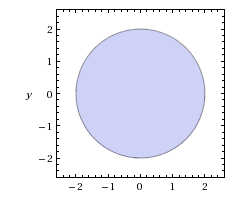
\includegraphics[scale = 0.75]{circle.png}
	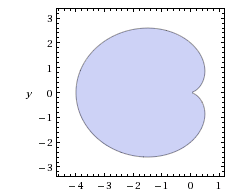
\includegraphics[scale = 0.75]{cardioid.png} \\
	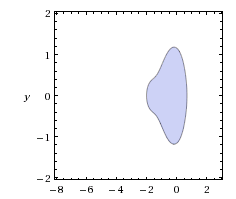
\includegraphics[scale = 0.75]{pear.png} 
	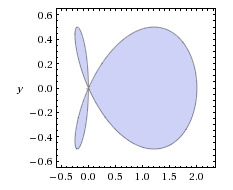
\includegraphics[scale = 0.75]{whale.png}	\\
	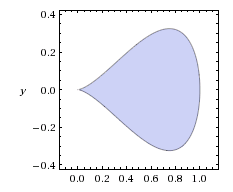
\includegraphics[scale = 0.75]{tear.png}
	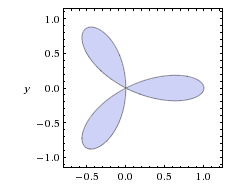
\includegraphics[scale = 0.75]{rose.png}
\end{center}	
	
\end{itemize}
W trakcie obliczeń co \textbf{interval} iteracji wyświetlana jest informacja o aktualnej wartości przybliżenia. Na koniec działania programu wyświetlany jest ostateczny wynik - wartość $S(f)$.
\section{Przykłady}
\begin{enumerate}
\item \textbf{Wywołanie:} \\
\verb|MonteCarlo(@(x,y)sqrt(x^2+y^2), 3, 10000000, 50000000, @(x,y)x^2+y^2-2^2, -2, 2, -2, 2, 0)|
\\\textbf{Wyjście:}
\\Wartosc po 10000000 iteracjach: 16.754448
\\Wartosc po 20000000 iteracjach: 16.758122
\\Wartosc po 30000000 iteracjach: 16.760322
\\Wartosc po 40000000 iteracjach: 16.757326
\\Wartosc po 50000000 iteracjach: 16.758204
\\\textbf{ans = } 16.758204480000000
\\\textbf{Wartość dokładna: $I(f) = 2\pi\cdot\frac{8}{3} = 16.755160819145$}

\item \textbf{Wywołanie:} \verb|MonteCarlo(@(x,y)1, 1, 10000000, 50000000, 0, 0, 0, 0, 0, 2)|
\\\textbf{Wyjście:}
\\Wartosc po 10000000 iteracjach: 18.836752
\\Wartosc po 20000000 iteracjach: 18.851856
\\Wartosc po 30000000 iteracjach: 18.853440
\\Wartosc po 40000000 iteracjach: 18.855974
\\Wartosc po 50000000 iteracjach: 18.856806
\\\textbf{ans = } 18.856806400000000
\\\textbf{Wartość dokładna: $I(f) = \frac{3\pi}{2} = 18.84955592153875943$}

\end{enumerate}
\end{document}
